\documentclass[border=5pt]{standalone}
\usepackage{tikz}
\usetikzlibrary{arrows.meta,positioning,fit}
\usepackage{lmodern}
\usepackage{xcolor}
\definecolor{navy}{HTML}{17365D}
\definecolor{teal}{HTML}{0F6B6D}
\definecolor{amber}{HTML}{B56B00}
\definecolor{softgray}{HTML}{F3F5F7}
\begin{document}
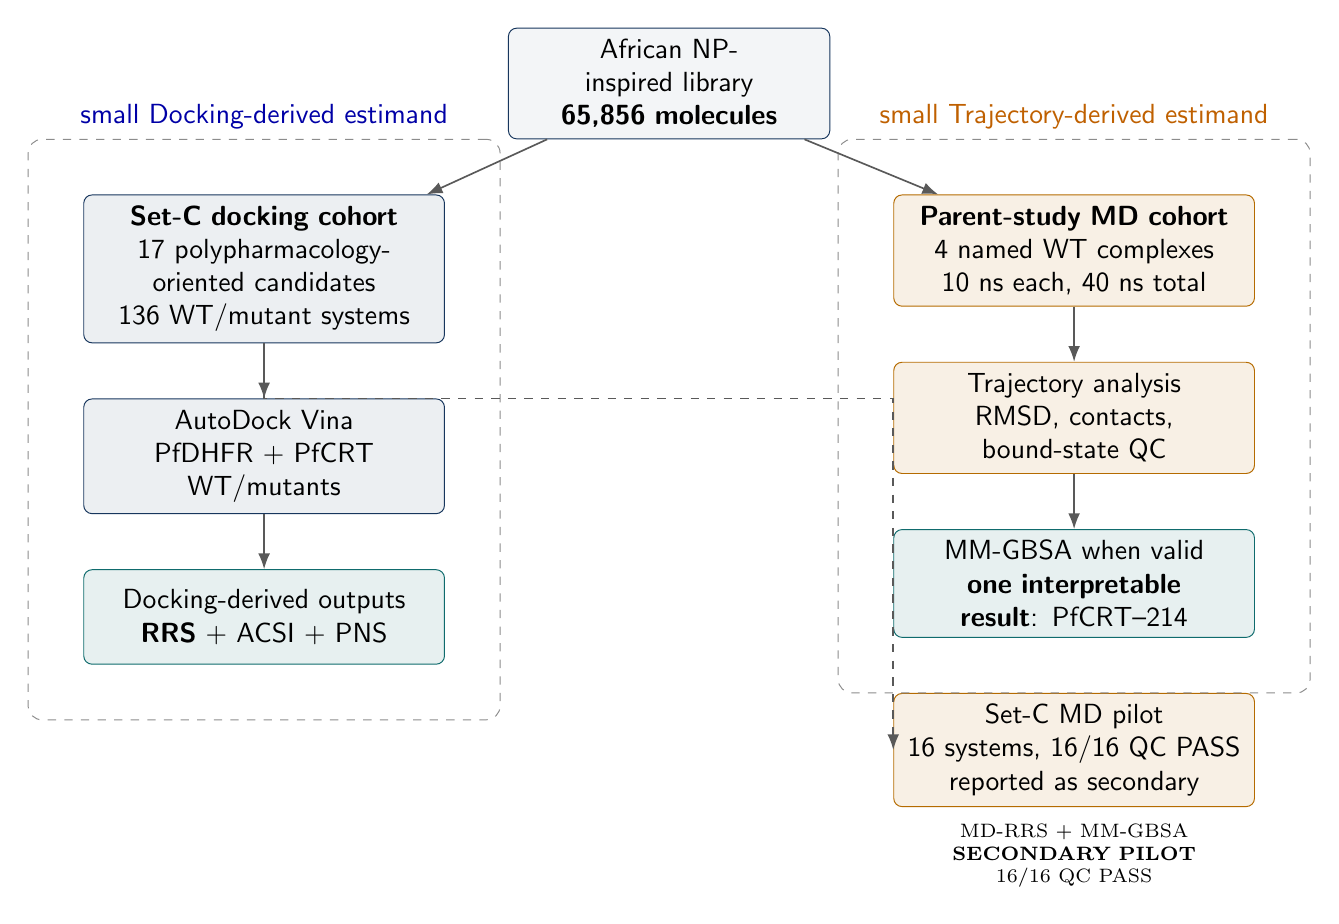
\begin{tikzpicture}[
  font=\sffamily,
  >=Latex,
  node distance=7mm and 8mm,
  every node/.style={line width=0.35pt},
  source/.style={draw=navy, rounded corners=3pt, fill=softgray, align=center, text width=38mm, minimum height=10mm, inner sep=4pt},
  dock/.style={draw=navy, rounded corners=3pt, fill=navy!8, align=center, text width=43mm, minimum height=12mm, inner sep=4pt},
  md/.style={draw=amber, rounded corners=3pt, fill=amber!10, align=center, text width=43mm, minimum height=12mm, inner sep=4pt},
  result/.style={draw=teal, rounded corners=3pt, fill=teal!10, align=center, text width=43mm, minimum height=12mm, inner sep=4pt},
  boundary/.style={draw=black!45, dashed, rounded corners=5pt, inner sep=7mm},
  arrow/.style={->, semithick, draw=black!65}
]

\node[source] (library) {African NP-inspired library\\\textbf{65,856 molecules}};
\node[dock, below left=of library] (setc) {\textbf{Set-C docking cohort}\\17 polypharmacology-oriented candidates\\136 WT/mutant systems};
\node[md, below right=of library] (parent) {\textbf{Parent-study MD cohort}\\4 named WT complexes\\10 ns each, 40 ns total};

\node[dock, below=of setc] (dockmetrics) {AutoDock Vina\\PfDHFR + PfCRT WT/mutants};
\node[result, below=of dockmetrics] (rrs) {Docking-derived outputs\\\textbf{RRS} + ACSI + PNS};
\node[md, below=of parent] (mdmetrics) {Trajectory analysis\\RMSD, contacts, bound-state QC};
\node[result, below=of mdmetrics] (mmgbsa) {MM-GBSA when valid\\\textbf{one interpretable result}: PfCRT--214};

\node[md, below=of mmgbsa] (pilot) {Set-C MD pilot\\16 systems, 16/16 QC PASS\\reported as secondary};
\node[boundary, fit=(setc) (dockmetrics) (rrs), label={[blue!65!black]above:\\small Docking-derived estimand}] (dockbox) {};
\node[boundary, fit=(parent) (mdmetrics) (mmgbsa), label={[orange!75!black]above:\\small Trajectory-derived estimand}] (mdbox) {};

\draw[arrow] (library) -- (setc);
\draw[arrow] (library) -- (parent);
\draw[arrow] (setc) -- (dockmetrics);
\draw[arrow] (dockmetrics) -- (rrs);
\draw[arrow] (parent) -- (mdmetrics);
\draw[arrow] (mdmetrics) -- (mmgbsa);
\draw[arrow, dashed] (setc.south) -- ++(0,-7mm) -| (pilot.west);
\node[align=center, text width=35mm, font=\scriptsize, below=1mm of pilot] {MD-RRS + MM-GBSA\\\textbf{SECONDARY PILOT}\\16/16 QC PASS};
\end{tikzpicture}
\end{document}
